\chapter{Applications diverses}

L'algèbre linéaire est utilisée dans un grand nombre de domaines.
Certaines applications ne font appel qu'aux notions couvertes dans ce manuel alors
que d'autres requièrent des notions plus avancées.  Dans ce chapitre, vous
trouverez plusieurs exemples d'applications de l'algèbre linéaire.

Tel que je l'ai mentionné dans la préface, j'aimerais remercir
Monsieur Joseph Khoury de l'Université d'Ottawa pour m'avoir
donné la permission d'utiliser et d'adapter les exemples d'applications de l'algèbre linéaire qui 
se trouve sur son site Internet.

% interpolation lagrangienne et matrice de vandermonde

\section{Équilibrage des réactions chimiques}

Les techniques de l'algèbre linéaire peuvent être utilisées pour
faire de qu'on appelle l'équilibrage des réactions chimiques\footnote{Un
exemple semblable se trouve sur la page \url{http://aix1.uottawa.ca/~jkhoury/chemistryf.htm}}.
Par exemple, considérons la combustion du propane (\cf{C3H8}), gaz qui est
utilisé dans la cuisson ainsi que pour le chauffage de certaine maisons.  
Lorsqu'on le combine avec l'oxygène (\cf{O2}), les produits de combustion sont
le gaz carbonique (\cf{CO2}) et l'eau (\cf{H2O}) ce qu'on écrit de la façon 
suivante:
\[
\ce{$w\,$C3H8 + $x\,$O2 -> $y\,$CO2 + $z\,$H2O }
\]
L'équilibrage des réactions chimique consiste à déterminer la valeur
des constantes $w, x, y, z$ qui font en sorte que le nombre d'atomes
d'un même type (hydrogène, oxygène et carbone) de chaque côté de
la flèche \ce{->} qui indique la transformation soit identique.
Par convention, on choisit des valeurs entières pour ces constantes.

Nous avons donc trois équations linéaires:
\[
\begin{matrix}[rrcl]
\cf{C}: & 3w &=& y \\
\cf{H}: & 8w &=& 2z \\
\cf{O}: & 2x &=& 2y + z
\end{matrix}
\]

Bien qu'il ne soit pas nécessaire d'utiliser la procédure de Gauss-Jordan
pour résoudre un système d'équations linéaires aussi simple, 
nous allons néanmoins l'utiliser pour mieux faire le lien avec ce que nous avons vu dans le cours.
Nous commençons par écrire le système d'équations linéaires dans une forme
plus familière
\[
\left\{
\begin{matrix}
&-& y && &+& 3w &=& 0 \\
&& &-& 2z &+& 8w &=& 0 \\
2x &-& 2y &-& z && &=& 0
\end{matrix}
\right.
\]
Nous avons donc un système d'équations linéaires \textbf{homogène} avec 3 équations et 4 inconnues;
nous savons, par le \reftheo{theoreme2} que nous aurons une infinité de solutions; 
une façon équivalente de dire ceci est que nous aurons donc au moins une variable libre.

Ceci nous donne\footnote{N.B. nous faisons plus que de simples
opérations élémentaires sur les lignes à chaque étape}
\[
\begin{matrix}
\begin{bmatrix}[rrrr|r]
0 & -1 & 0 & 3 & 0 \\
0 & 0  & -2 & 8 & 0 \\
2 & -2 & -1 & 0 & 0
\end{bmatrix}
& \quad\Rightarrow
\begin{matrix}
L_1 \leftrightarrow (-L_3) \\
L_2 \rightarrow -\frac12 L_2
\end{matrix}
\quad\Rightarrow\quad&
\begin{bmatrix}[rrrr|r]
2 & -2 & -1 & 0 & 0\\
0 & 0  & 1 & -4 & 0 \\
0 & 1 & 0 & -3 & 0
\end{bmatrix} \\
&
L_1 - L_2 +2L_3\rightarrow L_1 
\quad\Rightarrow\quad&
\begin{bmatrix}[rrrr|r]
2 & 0 & 0 & -10 & 0\\
0 & 0  & 1 & -4 & 0 \\
0 & 1 & 0 & -3 & 0
\end{bmatrix} \\
&\begin{matrix}
\frac12 L_1 \rightarrow L_1 \\
L_2 \leftrightarrow L_3
\end{matrix} \quad\Rightarrow\quad &
\begin{bmatrix}[rrrr|r]
1 & 0 & 0 & -5 & 0\\
0 & 1  & 0 & -3 & 0 \\
0 & 0 & 1 & -4 & 0
\end{bmatrix}
\end{matrix}
\]
Tel que nous l'avions prédit, nous avons une variable libre ($w$), que l'on peut paramétriser par $t$
et la solution est:
\[
\begin{matrix}
x &=& 5t \\
y &=& 3t \\
z &=& 4t \\
w &=& t
\end{matrix}
\]
Si on revient au problème du départ, le fait qu'on ait une variable libre
n'est pas surprenant: si on double (ou triple, ou prend un multiple quelconque)
le nombre de chaque type de molécules, l'équation de la réaction chimique devrait
être toujours valable.

Le choix du paramètre $t$ qui donne les plus petites valeurs entières
à toutes les variables est $t=1$. Avec ce choix, l'équation décrivant
la réaction chimique est
\[
\ce{C3H8 + 5 O2 -> 3 CO2 + 4 H2O }
\]
qui est la solution recherchée.

\subsection{Combustion incomplète}

La réaction de combustion précédente est une réaction complète en ce sens que
le produit de réaction contenait uniquement du dioxyde de carbone.
On peut parfois avoir une réaction incomplète où on a également du
monoxyde de carbone qui est produit:
\[
\ce{$w\,$C3H8 + $x\,$O2 -> $y\,$CO2 + $z\,$H2O + $v\,$CO}
\]
Le nombre d'équations étant déterminé par les éléments présents, nous aurons toujours
3 équations et 5 inconnues: nous aurons donc une variable libre supplémentaire.
Les équations sont:
\[
\begin{matrix}
\cf{C}: & 3w &=& y && &+& v \\
\cf{H}: & 8w &=& 2z \\
\cf{O}: & 2x &=& 2y &+& z &+& v
\end{matrix}
\]
Au lieu d'écrire le système d'équations linéaires dans la forme familière, où toutes
les inconnues sont du côté gauche du signe de l'égalité, écrivons-les en gardant
l'inconnue $v$ du côté droit du signe de l'égalité
\[
\left\{
\begin{matrix}
&-& y && &+& 3w &=& v \\
&& &-& 2z &+& 8w &=& 0 \\
2x &-& 2y &-& z && &=& v
\end{matrix}
\right.
\]
On a donc un système tout à fait semblable au précédent sauf que ce ne sera pas
un système homogène en général en raison de la variable libre $v$.  Il y a deux raisons
pour lesquelles nous avons choisi de l'écrire ainsi. Premièrement, ceci nous permet
de suivre exactement les mêmes étapes que précédemment pour résoudre le système (la
matrice des coefficients).  Deuxièmement, on sait que, lorsqu'on a des variables
libres, on les paramétrise par des scalaires \textit{et on les met de l'autre côté du signe
d'égalité}; c'est ce que nous avons fait immédiatement.   La solution est obtenue comme précédemment
\[
\begin{matrix}
\begin{bmatrix}[rrrr|r]
0 & -1 & 0 & 3 & v \\
0 & 0  & -2 & 8 & 0 \\
2 & -2 & -1 & 0 & v
\end{bmatrix}
& \quad\Rightarrow
\begin{matrix}
L_1 \leftrightarrow (-L_3) \\
L_2 \rightarrow -\frac12 L_2
\end{matrix}
\quad\Rightarrow\quad&
\begin{bmatrix}[rrrr|r]
2 & -2 & -1 & 0 & v\\
0 & 0  & 1 & -4 & 0 \\
0 & 1 & 0 & -3 & -v
\end{bmatrix} \\
&
L_1 - L_2 +2L_3\rightarrow L_1 
\quad\Rightarrow\quad&
\begin{bmatrix}[rrrr|r]
2 & 0 & 0 & -10 & -v\\
0 & 0  & 1 & -4 & 0 \\
0 & 1 & 0 & -3 & -v
\end{bmatrix} \\
&\begin{matrix}
\frac12 L_1 \rightarrow L_1 \\
L_2 \leftrightarrow L_3
\end{matrix} \quad\Rightarrow\quad &
\begin{bmatrix}[rrrr|r]
1 & 0 & 0 & -5 & -\frac12 v\\
0 & 1  & 0 & -3 & -v \\
0 & 0 & 1 & -4 & 0
\end{bmatrix}
\end{matrix}
\]
Nous avons donc deux variables libres; choisissons de paramétriser $w$ par t
comme précédemment; nous aurons
\[
\begin{matrix}
x &=& 5t &-&\frac12 v\\
y &=& 3t &-&v\\
z &=& 4t \\
w &=& t
\end{matrix}
\]
Ceci nous donne
\[
\ce{$t\,$C3H8 + $(5t-\frac{1}{2}v)\,$O2 -> $(3t-v)\,$CO2 + $4t\,$H2O + $v\,$CO}
\]

Écrivons $v=2st$ où $s$ est un paramètre arbitraire.  Ceci nous permet d'avoir
uniquement des valeurs entières pour les coefficients
\[
\ce{$t\,$C3H8 + $t(5-s)\,$O2 -> $t(3-2s)\,$CO2 + $4t\,$H2O + $2st\,$CO}
\]
De plus, on voit que chaque terme est multiplié par la variable libre $t$ comme précédemment, ce
que nous avions expliqué en indiquant que nous pouvons doubler ou tripler (etc.) 
la quantité des substances en jeu sans changer la réaction.  Faisons le choix $t=1$ comme
précédemment, ce qui nous donne
\[
\ce{C3H8 + $(5-s)\,$O2 -> $(3-2s)\,$CO2 + $4\,$H2O + $2s\,$CO}
\]
Mathématiquement, on ne peut pas en dire plus sur la valeur de la variable libre $s$.
Dans la pratique, cette valeur va dépendre des conditions physiques: alimentation en
air frais, évacuation des produits de combustion, etc. Comme le monoxyde de carbone
est un poison pour les humains, il est essentiel d'assurer une bonne alimentation
en air frais et une bonne ventilation des gaz de combustion pour les fournaises,
de façon à assurer une combustion complète!

\section{Courbes dans le plan}

Dans le chapitre précédent, nous avons étudié brièvement la géométrie vectorielle.  
Nous avons vu, entre autres, comment obtenir l'équation d'une droite dans l'espace.
Dans cette section, nous allons nous restreindre notre études aux courbes dans
le plan, et allons voir brièvement comment nous pouvons obtenir les équations
de courbes passant par des points définis. La méthode que nous allons
utiliser est différente de celle du chapitre précédent: nous allons uniquement
utiliser des propriétés des déterminants, sans utiliser les vecteurs\footnote{Ces exemples
ont été adaptés du site \url{http://aix1.uottawa.ca/~jkhoury/geometryf.htm}.}.

\subsection{Équation d'une droite dans le plan}

Commençons par l'exemple le plus simple, soit celui d'une droite. Soit deux points
\[
\begin{matrix}
P_1 &=& (x_1, y_1) &=& (1, -2)\\
P_2 &=& (x_2, y_2) &=& (-5, 2)
\end{matrix}
\]
 Nous voulons trouver les valeurs $a, b, c$ telles
que l'équation $ax+by+c=0$ est l'équation de la droite passant par ces deux points.
Nous savons que ceci est toujours possible, et que la solution n'est certainement pas
$a=b=c=0$; gardez ceci en tête.

Pour trouver cette solution, nous considérons un troisième point appartenant à cette
droite que nous allons dénoter ainsi:
\[
P = (x, y)
\]
À noter que nous ne connaissons pas, pour l'instant du moins, les valeurs
exactes des coordonnées $x, y$ de ce point; tout ce que nous savons est qu'il
existe et satisfait l'équation de la droite.   Nous avons donc le système d'équations
linéaires homogènes suivant
\[
\left\{
\begin{matrix}[lllllll]
ax &+& by &+& c &=& 0 \\
ax_1 &+& by_1 &+& c &=& 0 \\
ax_2 &+& by_2 &+& c &=& 0
\end{matrix}
\right.
\]
\textbf{où les inconnues recherchées sont } $a, b$ et $c$.  Une solution de ce système
est la solution $a=b=c=0$, ce qui n'est certainement pas la solution recherchée.
Comme nous savons qu'il existe  au moins une autre solution, celle de l'équation de la droite,
nous en concluons qu'il en existe une infinité de solutions et que les trois équations
linéaires ci-dessus sont linéairement dépendantes.  Ceci veut dire que le déterminant
de la matrice des 
coefficients\footnote{Rappelons que les inconnues du système d'équations linaires sont $a,b,c$.} est égal à zéro:
\[
\begin{vmatrix}[lll]
x & y & 1 \\
x_1 & y_1 & 1 \\
x_2 & y_2 & 1
\end{vmatrix} = 0
\]
En faisant l'expansion par la première ligne, on trouve
\[
x(y_1 - y_2) -y(x_1-x_2) + (x_1 y_2 - x_2 y_1) = 0
\]
En substituant les valeurs originales des points $P_1$ et $P_2$, nous trouvons
\[
-4x -6y -8 = 0
\]
Une solution possible est donc $a=-4, b=-6, c=-8$.  Une autre solution, 
totalement équivalent mais avec des coefficients plus simple, est
obtenue en divisant chacune de ces valeurs par $-2$ pour nous donner l'équation de la
droite:
\[
2x+3y+4 = 0
\]
On peut vérifier que la droite passe effectivement par les points $P_1$ et $P_2$.

\subsection{Équation d'un cercle dans le plan}

Soient les points $P_1 = (6,4)$, $P_2 = (-1,5)$ et $P_3 = (-3,1)$.  On désire
trouver l'équation du cercle qui passe par ces trois points.

\begin{figure}[h]
\begin{center}
\begin{tikzpicture}[>=stealth,scale=0.5]
	% les axes
	\draw[->,thin,black!70] (-4,0) -- (9,0) node[anchor=west]{x};
	\draw[->, thin,black!70] (0,-5) -- (0,8) node[anchor=south]{y};
	\coordinate [label=right:{\color{red}$(x_c,y_c)$}] (C) at (2, 1);
	\coordinate [label=right:{$P_1 = (6,4)$}] (P1) at (6, 4);
	\coordinate [label=left:{$P_2 = (-1,5)$}] (P2) at (-1,5);
	\coordinate [label=left:{$P_3 = (-3,1)$}] (P3) at (-3,1);
% initial area
	\draw[red] (C) circle (5cm);
	\filldraw[red] (C) circle (1mm);
	\filldraw[blue] (P1) circle (1mm);
	\filldraw[blue] (P2) circle (1mm);
	\filldraw[blue] (P3) circle (1mm);
\end{tikzpicture}
\caption{Unique cercle passant par trois points qui ne sont pas situés sur une droite.}
\end{center}
\end{figure}

L'équation d'un cercle de rayon $r$ dont le centre est situé au point $(x_c, y_c)$
est donnée par:
\[
(x-x_c)^2 + (y-y_c)^2 = r^2
\]
Donc, on cherche les valeurs des constantes $x_c, y_c, r$ qui font en sorte que
le cercle passera par les trois points donnés.
En faisant l'expansion des différents termes, on peut écrire ceci comme
\[
x^2 -2x x_c + x_c^2 + y^2 - 2y y_c + y_c^2 -r^2 = 0
\]
Ceci n'est pas une équation linéaire pour les inconnues $x_c, y_c, r$.  Ce qu'on
peut faire est introduire de nouvelles constantes $a,b,c,d$ telles que l'équation
ci-dessus peut être écrite sous la forme
\[
a(x^2+y^2) + bx + cy + d = 0
\]
qui est une équation linéaire.
On remarque que l'on a apparemment une constante superflue ($a$) qui devrait
être égale à 1 selon l'équation originale. En fait, ceci correspond, comme on
le verra sous peu, à la présence d'une variable libre dans le système à résoudre,
ce qui nous permet d'utiliser la méthode d'écrire un déterminant qui s'annule pour
obtenir l'équation recherchée.

Si on suppose que l'on a un quatrième point arbitraire, $(x,y)$ qui appartient à
ce cercle, on obtient un système d'équations linéaires homogène avec 4 équations
et 4 inconnues ($a,b,c,d$):
\[
\left\{
\begin{matrix}[lllllllll]
a(x^2+y^2) &+& bx &+& cy &+& d &=& 0 \\
a(x^2_1+y^2_1) &+& bx_1 &+& cy_1 &+& d &=& 0 \\
a(x^2_2+y^2_2) &+& bx_2 &+& cy_2 &+& d &=& 0 \\
a(x^2_3+y^2_3) &+& bx_3 &+& cy_3 &+& d &=& 0
\end{matrix}
\right.
\]
On sait que la solution triviale $a=b=c=d=0$ existe \ldots et qu'il y aura une
infinité de solutions si le déterminant de la matrice des coefficients
s'annule
\[
\begin{vmatrix}[llll]
(x^2+y^2) & x & y & 1\\
(x^2_1+y^2_1) & x_1 & y_1 & 1\\
(x^2_2+y^2_2) & x_2 & y_2 & 1\\
(x^2_3+y^2_3) & x_3 & y_3 & 1
\end{vmatrix}
=0
\]
Plutôt que d'obtenir l'équation générale, substituant les valeurs données initialement
et calculons ce déterminant
\[
\begin{vmatrix}[crrr]
(x^2+y^2) & x & y & 1\\
52 & 6 & 4 & 1\\
26 & -1 & 5 & 1\\
10 & -3 & 1 & 1
\end{vmatrix}
= (x^2+y^2) \begin{vmatrix}
 6 & 4 & 1\\
 -1 & 5 & 1\\
-3 & 1 & 1
\end{vmatrix} - x \begin{vmatrix}
52  & 4 & 1\\
26  & 5 & 1\\
10  & 1 & 1
\end{vmatrix} + y \begin{vmatrix}
52 & 6 & 1\\
26 & -1 & 1\\
10 & -3 &  1
\end{vmatrix} - \begin{vmatrix}
52 & 6 & 4 \\
26 & -1 & 5 \\
10 & -3 & 1 
\end{vmatrix} = 0
\]
En faisant les calculs on trouve
\[
30(x^2 + y^2) -120 x -60y -600 = 0
\]
Si on divise par 30, cette équation devient
\[
(x^2 + y^2) -4 x -2y -20 = 0
\]
qui est l'équation recherchée.  
En comparant avec l'équation du départ, on trouve que
\[
\begin{matrix}[rcl]
-4 = -2x_c &\Rightarrow& x_c = 2 \\
-2 = -2y_c &\Rightarrow& y_c = 1 \\
-20 = x_c^2 + y_c^2 - r^2 &\Rightarrow& r^2=25
\end{matrix}
\]
ce qui nous permet d'écrire
\[
(x-2)^2 + (y-1)^2 = 25
\]
On vérifiera que les trois points donnés satisfont cette équation.

\subsection{Mouvement des corps célestes}

Supposons que l'on observe un nouvel objet, tel que possiblement une comète, qui se dirige
vers l'intérieur du système solaire.  Si on néglige l'effet des planètes, le mouvement du
nouvel objet sera affecté par l'attraction gravitationnelle du Soleil\footnote{On peut toujours utiliser
la loi d'attraction gravitationnelle pour déterminer la trajectoire de l'objet si on tient compte de
la présence des planètes mais, dans ce cas, la trajectoire sera beaucoup plus compliqué qu'une simple
section conique.  De plus, sauf dans le cas où l'objet passerait tout près d'une planète, l'effet
de l'attraction gravitationnelle des planètes sur l'objet sera négligeable comparativement
à celui de l'attraction du Soleil.} et résultera en une trajectoire qui sera dans un plan et correspondra
à une section conique\footnote{La démonstration de ce fait requiert la résolution d'un système
d'équation différentielles non-linéaire du deuxième degré, ce qui est fait normalement dans un cours
de calcul différentiel et intégral de deuxième année universitaire.} (ellipse, parabole ou hyperbole).  
Si la vitesse de l'objet est inférieure à ce qu'on
appelle la vitesse d'échappement, la trajectoire suivie sera une ellipse; si la vitesse est supérieure
à la vitesse d'échappement, la trajectoire suivie sera une hyperbole.  

L'équation générale d'une section conique dans le plan peut être écrite sous la forme suivante:
\[
a x^2 + + bxy + cy^2 + dx + ey + f = 0
\]
Il s'agit donc d'une équation avec 6 inconnues.  Il suffit de déterminer la position de 5 points pour 
obtenir un système d'équations linéaires homogène avec 6 équations et 6 inconnues et de procéder comme
nous l'avons fait précédemment dans le cas de l'équation d'un cercle pour déterminer la valeur des inconnues.

Ce genre de calcul peut être très utile pour déterminer si la Terre sera frappée par un nouvel objet céleste
dont on détecterait la présence dans le système solaire!

\section{Série de Fourier}

Au chapitre \ref{chap:produit}, nous avons mentionné que l'espace des fonctions continues réelles 
sur l'intervalle $a\leq x \leq b$ était un espace vectoriel sur lequel
on pouvait définir un produit scalaire de la façon suivante:
\[
\langle f, g \rangle = \int_a^b f(x) g(x) dx
\]
Considérons l'intervalle $-L\leq x \leq L$. Pour cet intervalle, le mathématicien Jean Baptiste Joseph
Fourier (1768-1830) a démontré que l'ensemble des fonctions\footnote{Pour comprendre 
tous les aspects des séries de Fourier, il est essentiel
d'être familier avec le calcul différentiel et intégral; cependant, le lien avec les sujets traités dans
le cours d'algèbre linéaire, en particulier l'expansion en une combinaison linéaire des vecteurs
d'une base, devraient être suffisamment clairs même pour ceux qui sont peu familiers avec le calcul 
différentiel et intégral.}
\[
\left\{ \cos \frac{n\pi x}{L}, \sin \frac{n\pi x}{L} \right\}
\]
où $n$ désigne un entier, formait une base pour cet espace, et donc, qu'on pouvait représenter
toute fonction continue définie sur cet intervalle par une combinaison linéaire de ces fonctions.
De façon plus explicite, nous avons pour une fonction $f(x)$ 
\[
f(x) = \frac{a_0}{2} + \sum_{n=1}^\infty \left[a_n \cos \frac{n\pi x}{L} + b_n \sin \frac{n\pi x}{L}\right]
\]
avec
\[
\begin{matrix}
a_n &=&\displaystyle \frac{1}{L} \int_{-L}^L f(x) \cos \frac{n\pi x}{L} \, dx  &=& \langle f, \cos \frac{n\pi x}{L} \rangle \\
b_n &=&\displaystyle \frac{1}{L} \int_{-L}^L f(x) \sin \frac{n\pi x}{L} \, dx &=& \langle f, \sin \frac{n\pi x}{L} \rangle 
\end{matrix}
\]
Pour simplifier l'écriture, écrivons $\displaystyle C_n = \cos \frac{n\pi x}{L}, S_n = \sin \frac{n\pi x}{L}$
et $C_0 = \frac{1}{\sqrt{2}}$, ce qui nous permet d'écrire\footnote{À noter que $S_0 = 0$.}
\[
f(x) = \sum_{n=0}^\infty \big[ \langle f, C_n \rangle \mat{C}_n + \langle f, S_n \rangle \mat{S}_n \big]
\]
où l'on voit mieux l'expansion en terme des vecteurs de la base, avec les coefficients obtenus par
le produit scalaire.

\begin{figure}[h]
\begin{minipage}{0.45\textwidth}
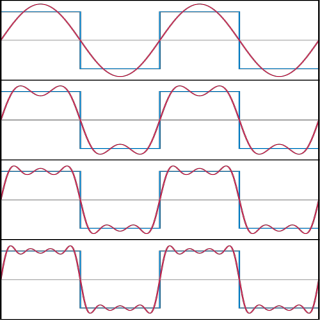
\includegraphics[width=\textwidth]{./images/fourier2}
\caption{Expansion partielle d'une fonction "onde carrée" en une série de Fourier. L'image
du haut inclut seulement le premier terme de la série et les autres
incluent respectivement les 2, 3 et 4 premiers termes de la série. Image adaptée de Wikipedia.
{\tiny \url{http://en.wikipedia.org/wiki/Fourier_series}}}
\end{minipage}\hfill
\begin{minipage}{0.5\textwidth}
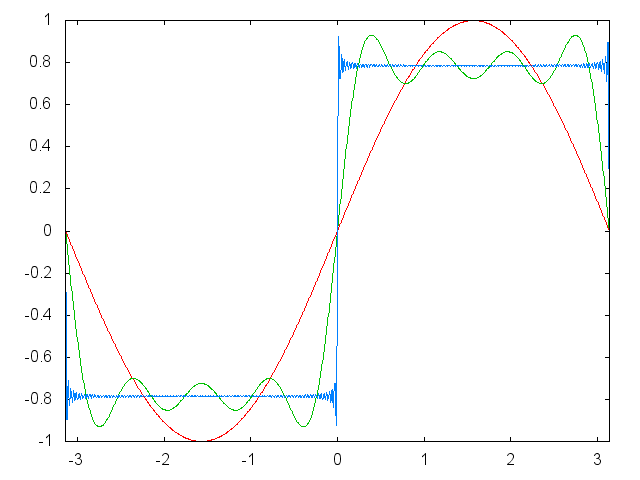
\includegraphics[width=\textwidth]{./images/fourier}
\caption{Série partielle de Fourier pour une fonction "onde carrée"
où l'on inclut le premier terme (en rouge), les quatre premiers termes (en vert), 
et les cent premiers (en bleu).}
\end{minipage}
\end{figure}

\subsection{Équations différentielles}

Les fonctions trigonométriques, qui forment la base de l'espace vectoriel pour les séries de Fourier,
obéissent l'équation différentielle suivante:
\[
\frac{d^2}{dx^2} f = -\frac{n^2\pi^2}{L^2} f \quad \Rightarrow \quad D^2 f = \lambda f
\]
c'est-à-dire qu'elles ont la forme requise\footnote{En dépit de l'exposant 2 qui apparait,
l'opérateur $D^2$ est un opérateur linéaire, c'est-à-dire qu'il obéit la relation
$D^2(af+bg) = a\,D^2f + b\,D^2g$ où $a,b$ sont des scalaires et $f,g$ sont des fonctions (donc, vecteurs
d'un espace vectoriel).} pour être des vecteurs propres d'un espace vectoriel.
En fait, plusieurs problèmes qui sont formulés comme des équations différentielles prennent une forme
semblable, et la connaissance de l'algèbre linéaire peut faciliter la recherche de solutions.

Par exemple, l'équation différentielle décrivant le mouvement de la peau d'un tambour circulaire
\[
\frac{\partial^2 \, f}{\partial t^2} = c^2 \left(\frac{\partial^2 \, f}{\partial x^2} + \frac{\partial^2 \, f}{\partial y^2}\right)
\]
peut également être reformulée comme un problème de recherche de vecteurs propres.

\subsection{Application à la musique}

Les séries de Fourier peuvent être utilisées pour décrire le mouvement périodique (dans le temps) de
la vibration des cordes de certains instruments de musique.  Les valeurs propres que l'on trouve sont
essentiellement les mêmes que données ci-dessus, on les exprimes généralement en fonction de la fréquence
de vibration, $f$; les diverses fréquences de  vibration obéissent la relation
\[
f_n = n f_1 \qquad n = 1, 2, 3, \ldots
\]
et sont appelées harmoniques, et la fréquence la plus basse, $f_1$, est appelée la fréquence fondamentale.
Parce que les harmoniques sont des multiples entiers, les sont qui résultent de combinaisons linéaires
des divers harmoniques sont jugées plaisants à notre oreille.

Par contre, les fréquences de vibration des divers modes de vibration (c'est-à-dire les vecteurs propres) d'une
peau de tambour ne sont pas des multiples entiers de la fréquence fondamentale.  Par conséquent,
notre oreille trouve que le son d'un tambour est moins harmonieux que celui d'un violon ou d'une guitare.
Vous pouvez visionner plusieurs mode de vibration d'une peau de tambour à la page Internet\\
\url{http://en.wikipedia.org/wiki/Vibrations_of_a_circular_membrane}

\section{Suite de Fibonacci}

La suite de Fibonacci\footnote{Cette section a été adaptée du site \url{http://aix1.uottawa.ca/~jkhoury/fibonaccif.htm}.
Voir également \url{http://fr.wikipedia.org/wiki/Suite_de_Fibonacci} pour plus de détails.}
\[
0, 1, 1, 2, 3, 5, 8, 13, \ldots 
\]
est une suite très connue d'entiers qui apparait dans beaucoup d'endroits, aussi bien dans la nature que dans
l'art et dans les sciences.  Les entiers de cette suite sont obtenus en additionnant les deux entiers
précédents pour obtenir le suivant, en commençant avec 0 et 1.  Ainsi, nous avons:
\[
\begin{matrix}[rcl]
f_0 &=& 0 \\
f_1 &=& 1 \\
f_2 &=& f_1 + f_0 = 0 + 1 = 1 \\
f_3 &=& f_2 + f_1 = 1 + 1 = 2 \\
f_4 &=& f_3 + f_2 = 2 + 1 = 3 \\
\vdots && \vdots \\
f_n &=& f_{n-1} + f_{n-2}
\end{matrix}
\]
Cette suite, d'apparence anodine, croit très rapidement; ainsi $f_{101} = 573147844013817084101$.

Une relation où un nombre, comme $f_n$ est obtenu à partir de nombres précédents est connue sous le 
nom de \textit{relation de récurrence}.  Une telle relation peut être exprimée sous forme matricielle.
Ainsi, on peut vérifier que
\[
\begin{pmatrix}
1 & 1 \\
1 & 0
\end{pmatrix} \begin{pmatrix}
f_{n-1} \\
f_{n-2}
\end{pmatrix}
=
\begin{pmatrix}[c]
f_{n-1} + f_{n-2} \\
f_{n-1}
\end{pmatrix}
=
\begin{pmatrix}[c]
f_n \\
f_{n-1}
\end{pmatrix}
\]
ce qu'on peut écrire comme
\[
\matA \begin{pmatrix}[c]
f_{n-1} \\
f_{n-2}
\end{pmatrix} = 
\begin{pmatrix}[c]
f_n \\
f_{n-1}
\end{pmatrix}
\]
On note que la matrice $\matA$ peut être écrite comme
\[
\matA = \begin{pmatrix}[cc]
f_2 & f_1 \\
f_1 & f_0
\end{pmatrix}
\]
On peut vérifier facilement que
\[
\matA^2 = \begin{pmatrix}
f_3 & f_2 \\
f_2 & f_1
\end{pmatrix}
\]
et, en fait, que
\[
\matA^n = \begin{pmatrix}[cc]
f_{n+1} & f_n \\
f_n & f_{n-1}
\end{pmatrix}
\]
\begin{exerciceC}
Démontrez que $\displaystyle \matA^n = \begin{pmatrix}[cc]
f_{n+1} & f_n \\
f_n & f_{n-1}
\end{pmatrix} $
\end{exerciceC}
Nous avons vu comment élever des matrices carrées à un large puissance en utilisant la diagonalisation.  Voyons
comment nous pouvons utiliser ceci pour obtenir une autre façon de calculer $f_n$.
Nous commençons par trouver le polynôme caractéristique:
\[
|\matA - \lambda \matI|   = 0  \quad\Rightarrow\quad \lambda^2 - \lambda -1 = 0  
\]
Nous trouvons deux solutions: $\lambda_\pm = \displaystyle\frac{1\pm \sqrt{5}}{2}$
À partir de ces valeurs propres, nous pouvons trouver deux vecteurs propres différents:
\[
\lambda_+ : \matX_+ = \begin{pmatrix}[cc]
\displaystyle \frac{1+ \sqrt{5}}{2} \\[10pt]
1
\end{pmatrix}
\qquad\qquad\lambda_- : \matX_- = \begin{pmatrix}[cc]
\displaystyle \frac{1- \sqrt{5}}{2} \\[10pt]
1
\end{pmatrix}
\]
et donc la matrice de passage est:
\[
\mat{P} = (\matX_+ \matX_-) = 
\begin{pmatrix}[cc]
\displaystyle \frac{1+ \sqrt{5}}{2} & \displaystyle \frac{1- \sqrt{5}}{2} \\[10pt]
1 & 1
\end{pmatrix}
\]
et son inverse est
\[
\mat{P}^{-1} = \frac{\sqrt{5}}{5}\begin{pmatrix}
1 & \displaystyle \frac{-1+ \sqrt{5}}{2} \\[10pt]
-1 & \displaystyle \frac{1+ \sqrt{5}}{2}
\end{pmatrix}
\]
Nous pouvons utiliser la matrice de passage et son inverse pour diagonaliser$\matA$:
\[
\mat{P}^{-1}\matA\mat{P} = \matD = \begin{pmatrix}[cc]
\displaystyle \frac{1+ \sqrt{5}}{2} & 0 \\[10pt]
0 & \displaystyle \frac{1 -\sqrt{5}}{2}
\end{pmatrix}
\]
Ainsi, nous avons
\[
\matD^n = 
\begin{pmatrix}[cc]
\displaystyle \left(\frac{1+ \sqrt{5}}{2}\right)^n & 0 \\[10pt]
0 & \left(\displaystyle \frac{1 -\sqrt{5}}{2}\right)^n
\end{pmatrix}
\]
ce qui nous permet de calculer
\[
\begin{matrix}[rcl]
\matA^n = \mat{P}\matD^n \mat{P}^{-1} &=& \displaystyle\frac{\sqrt{5}}{5}
 \begin{pmatrix}[cc]
 \displaystyle \frac{1+ \sqrt{5}}{2} & \displaystyle \frac{1- \sqrt{5}}{2} \\[10pt]
 1 & 1
 \end{pmatrix}
 \begin{pmatrix}[cc]
 \displaystyle \left(\frac{1+ \sqrt{5}}{2}\right)^n & 0 \\[10pt]
 0 & \left(\displaystyle \frac{1 -\sqrt{5}}{2}\right)^n
 \end{pmatrix}
 \begin{pmatrix}
 1 & \displaystyle \frac{-1+ \sqrt{5}}{2} \\[10pt]
 -1 & \displaystyle \frac{1+ \sqrt{5}}{2}
 \end{pmatrix}
 \\[30pt]
&=& 
\displaystyle\frac{\sqrt{5}}{5}
 \begin{pmatrix}[cc]
 \displaystyle \frac{1+ \sqrt{5}}{2} & \displaystyle \frac{1- \sqrt{5}}{2} \\[10pt]
 1 & 1
 \end{pmatrix} \begin{pmatrix}
\displaystyle \left(\frac{1+ \sqrt{5}}{2}\right)^n & \displaystyle\left(\frac{1+ \sqrt{5}}{2}\right)^{n-1} \\[10pt]
-\left(\displaystyle \frac{1 -\sqrt{5}}{2}\right)^n & -\left(\displaystyle \frac{1 -\sqrt{5}}{2}\right)^{n-1}
 \end{pmatrix}
 \\[30pt]
&=& \displaystyle\frac{\sqrt{5}}{5}
\begin{pmatrix}[cc]
\displaystyle \left[\left(\frac{1+ \sqrt{5}}{2}\right)^{n+1} - \left(\displaystyle \frac{1 -\sqrt{5}}{2}\right)^{n+1}\right] & 
\displaystyle \left[\left(\frac{1+ \sqrt{5}}{2}\right)^n - \left(\displaystyle \frac{1 -\sqrt{5}}{2}\right)^n\right] \\[10pt]
\displaystyle \left[\left(\frac{1+ \sqrt{5}}{2}\right)^n - \left(\displaystyle \frac{1 -\sqrt{5}}{2}\right)^n\right] & 
\displaystyle \left[\left(\frac{1+ \sqrt{5}}{2}\right)^{n-1} - \left(\displaystyle \frac{1 -\sqrt{5}}{2}\right)^{n-1}\right]
 \end{pmatrix} \\[30pt]
 &=& \begin{pmatrix}[cc]
 f_{n+1} & f_n \\
 f_n & f_{n-1}
 \end{pmatrix}
\end{matrix}
\]
d'où l'on obtient $f_n = \displaystyle\frac{\sqrt{5}}{5} \left[\left(\frac{1+ \sqrt{5}}{2}\right)^n 
- \left( \frac{1 -\sqrt{5}}{2}\right)^n\right]$ ce qui, avec la présence de divers facteurs de $\sqrt{5}$ peut
sembler surprenant puisque $f_n$ est un entier!

\section{Dynamique des populations}

La population du Cap Breton décroit alors que celle de la région de Halifax augmente. 
La Chouette tachetée du Nord est en déclin rapide, avec environ 7\% de perte annuelle de la population. 
Moins de 30 couples reproducteurs demeurent en Colombie-Britannique, 
et l'espèce devrait être disparue au Canada dans les prochaines années\footnote{In Trouble in Canada - 
The Northern Spotted Owl \url{http://cooperbeauchesne.com/upload/images/publications_1312796247.pdf}} 

Ces deux exemples de dynamique des population peuvent être modélisés en utilisant l'algèbre linéaire. 
Par exemple, supposons que l'on observe depuis plusieurs années que 5\% de la population de la région 
du Cap Breton migre vers la région métropolitaine de Halifax à chaque année (et donc 95\% reste au Cap Breton)
alors que 1\% de la population
va de la région métropolitaine de Halifax vers celle du Cap Breton\footnote{Ceci est évidemment un
modèle grandement simplifié; pour mieux modéliser, on devrait tenir compte de la migration des
sous-populations en fonction de l'âge, ainsi que des patrons de migration avec les autres régions
comme, par exemple, la migration vers les province de l'Ouest à la recherche des emplois, ainsi que
du nombre de décès et de naissance et du vieillissement de la population, etc.}. 
Le changement des populations respectives d'une année à l'autre sera donné par
\[
\begin{pmatrix}
0.99 & 0.05 \\
0.01 & 0.95
\end{pmatrix}
\begin{pmatrix}[c]
\cf{H}_0 \\
\cf{CB}_0
\end{pmatrix}
=
\begin{pmatrix}[c]
\cf{H}_1 \\
\cf{CB}_1
\end{pmatrix}
\]
Par exemple, si on retrouve
400k\footnote{k est abrégé de kilo, c'est-à-dire 1000.} personnes dans la région 
métropolitaine de Halifax et 150k personnes dans celle du Cap Breton une certaine année,
l'année suivante, on aura:
\[
\begin{pmatrix}
0.99 & 0.05 \\
0.01 & 0.95
\end{pmatrix}
\begin{pmatrix}
400 \\
150
\end{pmatrix}
=
\begin{pmatrix}
403.5 \\
146.5
\end{pmatrix}
\]
et donc on verra un changement net de 3500 personnes dans chaque région.  Si cette
tendance se maintien pendant plusieurs années, 5\% de la région du Cap Breton représentera
un nombre de plus en plus petit de personne alors que 1\% de la région métropolitaine
de Halifax représentera un nombre de plus en plus grand; éventuellement ces deux nombres
pourraient, en principe, devenir égaux, et on aurait une situation en équilibre où
le nombre de personnes qui migre d'une région à l'autre est le même dans les deux sens:
\[
\begin{pmatrix}
0.99 & 0.05 \\
0.01 & 0.95
\end{pmatrix}
\begin{pmatrix}[c]
\cf{H}_n \\
\cf{CB}_n
\end{pmatrix}
=
\begin{pmatrix}[c]
\cf{H}_{n+1} \\
\cf{CB}_{n+1}
\end{pmatrix}
=
\begin{pmatrix}[c]
\cf{H}_n \\
\cf{CB}_n
\end{pmatrix}
\]
On reconnait ceci comme un problème de recherche de vecteur propre, avec une valeur propre égale à 1.
La matrice pour laquelle on recherche des vecteurs propres a la forme
\[
\begin{pmatrix}[cc]
1-a & b \\
a & 1-b
\end{pmatrix}
\]
Si on écrit $c=a+b$, on peut vérifier que son polynôme caractéristique est
\[
\lambda^2 - (2-c)\lambda + (1-c) = (\lambda -1)(\lambda -[1 - c]) = 0
\]
Le vecteur propre appartenant à la valeur propre $\lambda=1$ obéira l'équation
\[
\begin{pmatrix}
-a & b \\
a & -b
\end{pmatrix}\begin{pmatrix}[c]
\cf{H} \\ \cf{CB}
\end{pmatrix}= \begin{pmatrix}
0 \\ 0
\end{pmatrix}
\]
et on aura $a\,\cf{H} = b\, \cf{CB}$.  Puisque $a=0,01$ et $b=0,05$, on trouvera que
l'équilibre sera atteint lorsqu'on aura 5 fois plus de personnes dans la région
métropolitaine de Halifax que dans la région du Cap Breton\footnote{Soit approximativement
460k \textit{vs} 90k, arrondi au 10k près.}\ldots  ce qui
est un résultat évident lorsqu'on n'a que deux régions à tenir compte et lorsque
l'on suppose que la population demeure constante.  Par contre, lorsqu'on
a un modèle plus compliqué, la modélisation par multiplication de matrices
et la recherche de solution en utilisant les vecteurs propres est une
méthode qu'on peut toujours utiliser.

Par exemple, pour les chouettes tachetées, le modèle utilisé est le suivant
\footnote{Ce modèle est inspiré de 
\url{http://online.redwoods.cc.ca.us/instruct/darnold/laproj/Fall97/Asher/mike.pdf}}:
\begin{itemize}
\item On modélise l'évolution de la population sur une base annuelle, c'est-à-dire
qu'on prédit la population à l'année $N$ à partir de la population à l'année $N-1$.
\item On considère trois stages de vie: juvénile $J$ (un an ou moins),
sous-adulte $S$ (de un à deux ans) et adulte $A$ (deux ans et plus);
\item La proportion de juvéniles qui naissent par rapport au nombre
d'adulte est donné par le taux de reproduction $r$; donc $J_n = r A_{n-1}$.
\item Le taux de survie d'une année à l'autre est indiqué par la variable $t$.
Ainsi, le taux de survie des juvéniles (qui deviennent des sous-adultes) obéit
$S_n = t_J J_{n-1}$. Le nombre d'adulte pour l'année $N$ est une combinaison
du nombre de sous-adultes qui survivent (et deviennent des adultes) ainsi que
du nombre d'adultes qui survivent:
\[
A_n = t_S S_{n-1} + t_A A_{n-1}
\]
\end{itemize}
On peut écrire ceci sous forme matricielle de la façon suivante:
\[
\matA\mat{v} = 
\begin{pmatrix}
0 & 0 & r \\
t_J & 0 & 0 \\
0 & t_S & t_A
\end{pmatrix}
\begin{pmatrix}
J_{n-1}\\
S_{n-1} \\
A_{n-1}
\end{pmatrix}
=
\begin{pmatrix}
J_n \\
S_n \\
A_n
\end{pmatrix}
\]
où $\matA$ est la matrice de transition qui aura des
valeurs comme $r=0.3$, $t_j = 0.2$, $t_s=0.7$, $t_A=0.9$.
Supposons que l'on exprime le vecteur $\transp{(J, S, A)}$ comme une combinaison linéaire
des vecteurs propres de la matrice de transition
\[
\begin{pmatrix}
J\\S\\A
\end{pmatrix}
= a_1 \mat{v}_1 + a_2 \mat{v}_2 + \ldots
\]  Si on fait l'évolution dans le temps
sur plusieurs années, c'est-à-dire qu'on multiplie la matrice de transition à plusieurs reprises,
chaque vecteur propre de la combinaison linéaire sera multiplié par sa valeur propre à chaque fois
\[
\matA^n
\begin{pmatrix}
J\\S\\A
\end{pmatrix}
= a_1 \lambda_1^n \mat{v}_1 + a_2 \lambda_2^n \mat{v}_2 + \ldots
\]
Éventuellement, le terme qui deviendra dominant sera celui qui correspond à la valeur propre la
plus élevée (qu'on appelle la valeur propre dominante).  Si la valeur propre dominante est
plus grande que 1, alors le terme croitra et donc la population totale croitra également.
Par contre, si la valeur propre dominante est plus petite que 1, alors, lorsqu'on la multipliera
par elle-même, le résultat sera de plus en plus petit; par conséquent, ceci indique que la population
connaitra un déclin.

En changeant les conditions environnementales, on peut modifier les variables $t_J, t_S, t_A$ et
affecter soit la survie ou le déclin d'une population animale.

\section{Visages propres}

Les \textbf{visages propres} sont une application intéressante de l'algèbre linéaire et de la statistique.
Avant d'aborder une description des visages propres comme tel, je vais expliquer certains concepts
de façon graphique. Je dois noter que cet exemple provient du cours 
\textit{Machine Learning} que j'ai suivi et qui est offert gratuitement (sans crédits) sur Internet
par le professeur Andrew Ng de l'université Stanford aux États-Unis.



\begin{adjmulticols}{1}{0in}{-2in}

\begin{center}
\begin{minipage}{0.9\textwidth}
Nous allons commencer avec un exemple beaucoup plus simple, soit celui d'une distribution de
points dans le plan.
On peut voir que ces points ne sont pas distribués de façon
uniforme, mais semble être un peu aligné le long d'un axe
diagonal.
\end{minipage}
\hfill
\begin{minipage}{0.45\textwidth}
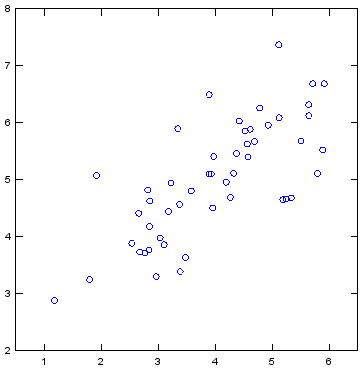
\includegraphics[width=\linewidth]{./images/pca_points}
\end{minipage}
\end{center}


\begin{center}
\begin{minipage}{0.9\textwidth}
À l'aide d'une méthode faisant appel à la statistique et connue sous le nom 
d'\textit{analyse de composantes principales} on peut identifier une direction
principale le long de laquelle les données sont alignées dans le plan,
ainsi qu'une direction secondaire. Ces deux directions orthogonales
vont être utilisées comme deux vecteurs de base, $\mat{v}_1$ et $\mat{v}_2$,
chaque point pouvant être représenté par des une combinaison linéaire
des vecteurs de cette base.
\end{minipage}
\hfill
\begin{minipage}{0.45\textwidth}
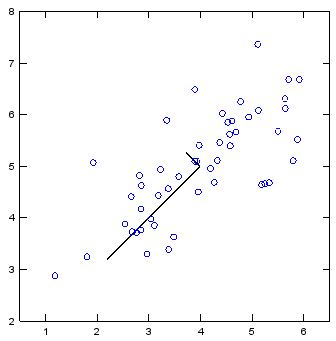
\includegraphics[width=\linewidth]{./images/pca_points2}
\end{minipage}
\end{center}


\begin{center}
\begin{minipage}{0.9\textwidth}
On utilise ces vecteurs de base pour construire des matrices de projection
pour laquelle ces vecteurs sont des vecteurs propres.  En utilisant ces
matrices de projection (équivalente au produit scalaire habituel), on peut
obtenir la décomposition d'un point en une combinaison linéaire des vecteurs
propres. En ne retenant qu'une seule des deux composantes, on obtient
une distribution approximative (indiquée en rouge) en une dimension de la distribution
originale (indiquée en bleu).  
\end{minipage}
\hfill
\begin{minipage}{0.45\textwidth}
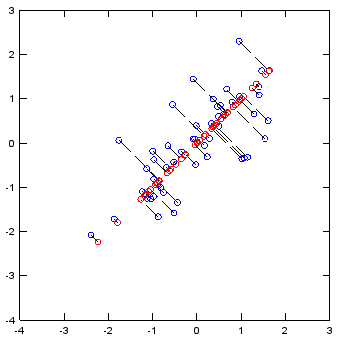
\includegraphics[width=\linewidth]{./images/pca_points3}
\end{minipage}
\end{center}

\end{adjmulticols}

Au lieu de simplement faire une approximation à une dimension d'une distribution de points
dans un espace à deux dimensions, nous allons approximer des points dans un espace
à 1024 dimensions, c'est-à-dire une distributions
de points dans $\BBR^{1024}$.



\begin{adjmulticols}{1}{0in}{-2in}

\begin{center}
\begin{minipage}{0.9\textwidth}
L'exemple choisi est celui de visages en niveaux de gris.
Nous commençons avec une collection de 5000 images de la même taille,
dont les cent premières sont montrées ici.  Notez que l'orientation des visages
est assez arbitraire et qu'aucun effort particulier n'a été fait pour les rendre
plus uniformes.
\end{minipage}
\hfill
\begin{minipage}{0.45\textwidth}
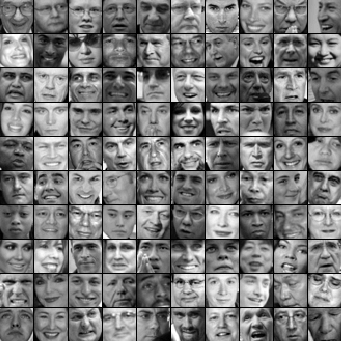
\includegraphics[width=\linewidth]{./images/faces}
\end{minipage}
\end{center}

\begin{center}
\begin{minipage}{0.9\textwidth}
Chaque image est formée de 1024 pixels organisés dans un carré,
donc de taille $32\times 32$. L'image à la droite correspond
à celle de la troisième ligne et sixième colonne de la collection
précédente et ressemble étrangement à Bill Clinton, ancien
président des États-Unis.

À partir de cette image, on peut former un vecteur de $\BBR^{1024}$
dont la première coordonnée correspond au niveau de gris (un nombre entre 0
et 255) pour le premier pixel en haut à gauche, et la dernière coordonnée
correspond à la valeur du pixel en bas à droite.
\end{minipage}
\hfill
\begin{minipage}{0.45\textwidth}
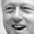
\includegraphics[width=\linewidth]{./images/clint1}
\end{minipage}
\end{center}

\begin{center}
\begin{minipage}{0.9\textwidth}
À partir des 5000 vecteurs, on fait l'analyse numérique pour trouver
les composantes principales qui deviendront les vecteurs de base
qu'on désigne sous le nom de \textit{visages propres}, ou 
\textit{eigenfaces} en anglais.

En ordre d'importance (en commençant en haut à gauche), on voit
les 36 premiers visages propres.   Faire la décomposition en composantes principales
pour ces 500 images
requiert environ une minute sur un ordinateur PC acheté en 2012.  Si on augmentait 
la taille des images, disons à 256 pixels par 256 pixels, on aurait besoin d'environ
une heure pour obtenir la même information; il y a 10 ans, le même calcul aurait pris plus
d'une journée sur un ordinateur PC.
\end{minipage}
\hfill
\begin{minipage}{0.45\textwidth}
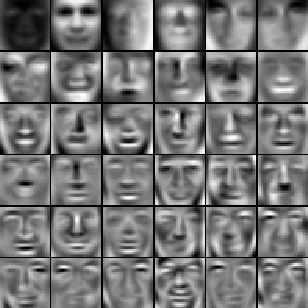
\includegraphics[width=\linewidth]{./images/faces_propres}
\end{minipage}
\end{center}


\begin{center}
\begin{minipage}{0.4\textwidth}
Comparaison entre la collection d'images originales
et celles formées par les combinaisons linéaires des
10 visages propres dominants.  On ne peut pas vraiment reconnaitre
les images originales à partir des combinaisons linéaires de 10 visages
propres.
\end{minipage}
\hfill
\begin{minipage}{0.45\textwidth}
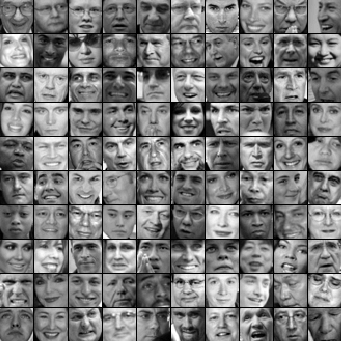
\includegraphics[width=\linewidth]{./images/faces}
\end{minipage}
\hfill
\begin{minipage}{0.45\textwidth}
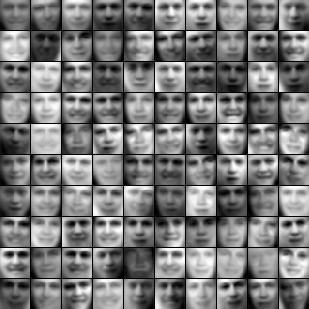
\includegraphics[width=\linewidth]{./images/faces10}
\end{minipage}
\end{center}

\begin{center}
\begin{minipage}{0.4\textwidth}
Comparaison entre la collection d'images originales
et celles formées par les combinaisons linéaires des
30 visages propres dominants.  Les images formées des combinaisons
linéaires commencent à ressembler davantage aux images originales,
mais toujours pas suffisamment pour qu'on puisse toutes les reconnaitre.
\end{minipage}
\hfill
\begin{minipage}{0.45\textwidth}
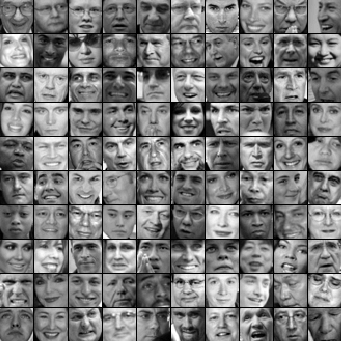
\includegraphics[width=\linewidth]{./images/faces}
\end{minipage}
\hfill
\begin{minipage}{0.45\textwidth}
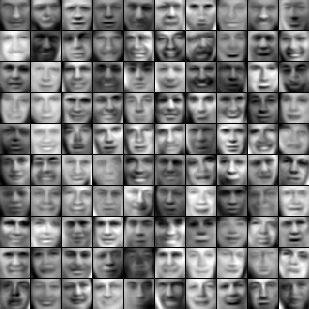
\includegraphics[width=\linewidth]{./images/faces30}
\end{minipage}
\end{center}

\begin{center}
\begin{minipage}{0.4\textwidth}
Comparaison entre la collection d'images originales
et celles formées par les combinaisons linéaires des
100 visages propres dominants.  On voit une très grande
ressemblance pour la plupart des images entre les 
combinaisons linéaires de 100 visages propres (des
vecteurs dans un espace à 100 dimensions) et les images originales qui sont des vecteurs dans
un espace à 1024 dimensions. Le temps requis pour calculer les 5000 combinaisons
linéaires de 100 visages propres est inférieur à une seconde.
\end{minipage}
\hfill
\begin{minipage}{0.45\textwidth}
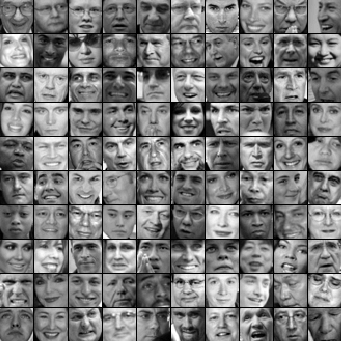
\includegraphics[width=\linewidth]{./images/faces}
\end{minipage}
\hfill
\begin{minipage}{0.45\textwidth}
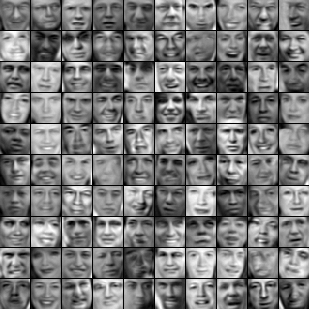
\includegraphics[width=\linewidth]{./images/faces_rec}
\end{minipage}
\end{center}


\begin{center}
\begin{minipage}{0.4\textwidth}
Comparaison entre une image originale particulière et la combinaison
linéaire de 100 visages propres.  En utilisant seulement 100 vecteurs,
au lieu de 1024 qui serait la base de l'espace en entier, on obtient
une réduction (compression des images) par un facteur supérieur à 10
tout en ayant une image assez semblable à l'originale.
\end{minipage}
\hfill
\begin{minipage}{0.45\textwidth}
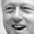
\includegraphics[width=\linewidth]{./images/clint1}
\end{minipage}
\hfill
\begin{minipage}{0.45\textwidth}
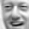
\includegraphics[width=\linewidth]{./images/clint2}
\end{minipage}
\end{center}

\end{adjmulticols}

En résumé, nous avons utilisé une collection de 5000 images, chacune pouvant être représentée par
un vecteur dans $\BBR^{1024}$ pour obtenir des vecteurs de base d'un espace $\BBR^{100}$ à partir
desquels on peut faire des combinaisons linéaires qui donnent une assez bonne approximation des images
originales.  La réduction du nombre de paramètres pour représenter les images est utile
pour deux types d'applications.  Premièrement, on peut se servir de ceci comme d'une méthode de compression
des images, ce qui, par exemple, peut réduire le temps de transmission (si on envoie ces images par Internet)
ou réduit l'espace requis pour l'entreposage.  Deuxièmement, on peut se servir de ceci pour des logiciels
d'identification de personnes automatisés; de tels logiciels sont beaucoup plus efficaces lorsqu'ils ont moins de paramètres
à évaluer pour faire une identification.


\section{Régression linéaire}

La régression linéaire
est un sujet normalement rencontré pour la première fois dans un cours
d'introduction à la statistique.  La présentation habituelle utilise des techniques de calcul
différentiel et intégral plutôt que d'algèbre linéaire et il peut être difficile de voir
ce qui se passe exactement.  Dans cette section, nous allons présenter la régression linéaire
en utilisant uniquement des techniques couvertes dans ce manuel, et donc sans faire appel
au calcul différentiel et intégral.  

Commençons par une mise en situation.

\begin{center}
\begin{minipage}{0.45\textwidth}
Il est impossible de tracer une droite qui passe par les points (1,1), (2,3) et (3,3).
Comment peut-on déterminer quelle serait la meilleure droite correspondant à ces points 
si on a un modèle qui prédit qu'ils devraient
en principe être alignés le long d'une droite?
\end{minipage}\hfill
\begin{minipage}{0.45\textwidth}
	\begin{tikzpicture}
	% les axes
	\draw[->] (-0.5,0) -- (3.5,0) node[anchor=west]{x};
	\draw[->] (0,-0.5) -- (0,3.5) node[anchor=south]{y};
	\fill [blue] (1,1) circle (2pt);
	\fill [blue] (2,3) circle (2pt);
	\fill [blue] (3,3) circle (2pt);
	\draw[-] (1,-0.1) node[anchor=north]{\tiny 1} -- (1, 0.1);
	\draw[-] (2,-0.1) node[anchor=north]{\tiny 2} -- (2, 0.1);
	\draw[-] (3,-0.1) node[anchor=north]{\tiny 3} -- (3, 0.1);
	\draw[-] (-0.1,1) node[anchor=east]{\tiny 1} -- (0.1, 1);
	\draw[-] (-0.1,2) node[anchor=east]{\tiny 2} -- (0.1, 2);
	\draw[-] (-0.1,3) node[anchor=east]{\tiny 3} -- (0.1, 3);
	\end{tikzpicture}
\end{minipage}
\end{center}

L'équation d'une droite non-verticale dans le plan $xy$ peut être écrite comme étant
$a_0 + a_1 x = y$.  Ainsi, si nous avons trois points qui appartiennent à cette droite
nous aurons le système d'équations linéaires suivant:
\[
\left\{
\begin{matrix}
a_0 + a_1 x_1 &=& y_1 \\
a_0 + a_1 x_2 &=& y_2 \\
a_0 + a_1 x_3 &=& y_3 \\
\end{matrix}
\right.
\]
\textbf{où les inconnues sont $a_0$ et $a_1$.}
On peut écrire ce système comme représentant une combinaison linéaire:
\[
a_0 \mathds{1} + a_1\matX = \matY
\]
où $\mathds{1}$ est un vecteur colonne dont tous les coefficients sont identiques
et égaux à 1.  En utilisant la notation matricielle pour présenter le problème comme
celui d'une combinaison linéaire, la généralisation à plus de trois points est immédiate.

Le cas qui nous intéresse est celui où $\matY$ ne peut \textbf{pas} être représenté comme
une combinaison linéaire des vecteurs $\mathds{1}$ et $\matX$.  Dans ce cas, on veut
trouver la \textbf{meilleure} combinaison linéaire possible, ce qui requiert que l'on
définisse ce qu'on entend par le mot \textbf{meilleure}.  On peut faire ceci
graphiquement.  Les vecteurs $\mathds{1}$ et $\matX$ de $\BBR^n$ engendrent un plan dans
$\BBR^n$.  Si le vecteur  $\matY$ peut être écrit comme une combinaison des vecteurs
$\mathds{1}$ et $\matX$, c'est qu'il appartient à ce plan; sinon, c'est qu'il n'appartient
pas à ce plan tel qu'illustré à la figure \ref{fig:nonplan}.

\begin{figure}[h]
\begin{tikzpicture}
	\coordinate  (A0) at (0, 0);
	\coordinate (B0) at (3, 3);
	\coordinate (C0) at (9, 0);
	\coordinate (D0) at (11.5, 3);
	\coordinate [label=right:{$\matY$}] (Y) at (7, 5);
	\coordinate  (O) at (4, 1);
	\coordinate [label=left:{$\mathds{1}$}] (One) at (3, 2);
	\coordinate [label=right:{$\matX$}] (X) at (8,1);
%	\coordinate [label=right:{\color{red} $\matZ$}] (C) at (7,2);
\begin{pgfonlayer}{background}
   \path [fill=blue!10] (A0) -- (B0) -- (D0) -- (C0) -- (A0);
\end{pgfonlayer}
%	\draw[dashed, black] (C) -- (Y);
% 	\draw[-] (6.56,1.83) -- (6.56,2.25);
% 	\draw[-] (6.56,2.25) -- (7,2.4);
% 	\draw[->, ultra thick, red] (O) -- (C);

	\draw[->,ultra thick,black] (O) -- (Y);
	\draw[->,ultra thick,blue] (O) -- (X);
	\draw[->,ultra thick,blue] (O) -- (One);
	\filldraw (O) circle (0.7mm);
%	\draw[dashed,blue] (One) -- (C);
%	\draw[dashed, blue] (X) -- (C);
\end{tikzpicture}
\caption{\label{fig:nonplan}
Le vecteur  $\matY$ n'appartient pas au plan engendré par les vecteurs 
$\mathds{1}$ et $\matX$.
}
\end{figure}

Par contre, comme on a vu dans le chapitre sur la géométrie vectorielle
lorsqu'on a calculé la distance d'un point a un plan, le point (vecteur) qui
appartient au plan engendré par les vecteurs $\mathds{1}$ et $\matX$
et qui est le plus proche au vecteur $\matY$ correspond à la projection
orthogonale du vecteur $\matY$ sur le plan, tel qu'illustré
à la figure \ref{fig:oui-plan}.

\begin{figure}[h]
\begin{tikzpicture}
	\coordinate  (A0) at (0, 0);
	\coordinate (B0) at (3, 3);
	\coordinate (C0) at (9, 0);
	\coordinate (D0) at (11.5, 3);
	\coordinate [label=right:{$\matY$}] (Y) at (7, 5);
	\coordinate  (O) at (4, 1);
	\coordinate [label=left:{$\mathds{1}$}] (One) at (3, 2);
	\coordinate [label=right:{$\matX$}] (X) at (8,1);
	\coordinate [label=right:{\color{red} $\matZ$}] (C) at (7,2);
\begin{pgfonlayer}{background}
   \path [fill=blue!10] (A0) -- (B0) -- (D0) -- (C0) -- (A0);
\end{pgfonlayer}
	\draw[dashed, black] (C) -- (Y);
 	\draw[-] (6.56,1.83) -- (6.56,2.25);
 	\draw[-] (6.56,2.25) -- (7,2.4);
 	\draw[->, ultra thick, red] (O) -- (C);

	\draw[->,ultra thick,black] (O) -- (Y);
	\draw[->,ultra thick,blue] (O) -- (X);
	\draw[->,ultra thick,blue] (O) -- (One);
	\filldraw (O) circle (0.7mm);
	\draw[dashed,blue] (One) -- (C);
	\draw[dashed, blue] (X) -- (C);
\end{tikzpicture}
\caption{\label{fig:oui-plan}
Le vecteur  $\matZ$, qui appartient au plan engendré par les vecteurs 
$\mathds{1}$ et $\matX$, est le vecteur de ce plan qui est la meilleure
approximation du vecteur
$\matY$, c'est-à-dire celui dont la distance $\norm{\matZ - \matY}$
est la plus petite.
}
\end{figure}
Donc la solution recherchée $(a_0, a_1)$ est celle qui satisfait
$a_0 \mathds{1} + a_1\matX = \matZ$ au lieu de $a_0 \mathds{1} + a_1\matX = \matY$.
On note que le vecteur $\matY - \matZ$, est perpendiculaire au plan engendré par
$\mathds{1}$ et $\matX$ et donc que le produit scalaire\footnote{On représente le
produit scalaire par le symbole $\cdot$ comme on l'avait fait au chapitre
sur la géométrie vectorielle.} 
\[
\matZ \cdot (\matY -\matZ) = 0
\]
Introduisons la matrice $\matM$ qui est formée des vecteurs colonnes qui génère le plan
\[
\matM = (\mathds{1} \matX) = \begin{pmatrix}
1 & x_1 \\
1 & x_2 \\
1 & x_3
\end{pmatrix}
\]
et le vecteur des inconnues
\[
\matA = \begin{pmatrix}
a_0 \\ a_1
\end{pmatrix}
\]
ce qui nous permet d'écrire
\begin{equation}
\matM\matA = \matZ \label{eq:Z}
\end{equation}
On se rappelle que le produit scalaire de deux vecteurs est obtenu
en prenant la transposée de l'un multipliée par l'autre (et où la
trace du résultat est sous-entendue):
\[
\matZ \cdot (\matY -\matZ) = 0 \qquad\Rightarrow\qquad \transp{\matZ} (\matY -\matZ) = 0
\]
En substituant la valeur pour $\matZ$ de l'équation \refeq{eq:Z}, on a
\[
\transp{(\matM\matA)} (\matY - \matM\matA) = 0
\]
Puisque $\transp{\matC\matD} = \transp{\matD}\transp{\matC}$, ceci devient
\[
\transp{\matA}\transp{\matM} (\matY - \matM\matA) = 0
\]
que l'on peut récrire sous la forme du produit scalaire suivant:
\[
\matA\cdot[\transp{\matM} (\matY - \matM\matA)] = 0
\]
Cette équation doit être vérifiée pour tous les vecteurs inconnus $\matA$; ceci veut dire que le vecteur
\[
\transp{\matM} (\matY - \matM\matA)
\]
doit s'annuler.  Nous devons donc avoir 
\begin{equation}
\transp{\matM} \matY =  \transp{\matM}\matM\matA \label{eq:regression}
\end{equation}
Ceci nous donne un système d'équations qu'on peut résoudre et qui ne dépend que des données du problème initial,
et non d'un vecteur inconnu comme $\matZ$.
Par exemple, si nous revenons au problème mentionné au tout début de la section de ce chapitre, nous avons:
\[
\matM = \begin{pmatrix}
1 & x_1 \\
1 & x_2 \\
1 & x_3
\end{pmatrix} = \begin{pmatrix}
1 & 1 \\
1 & 2 \\
1 & 3
\end{pmatrix}
\]
et
\[
\matY = \begin{pmatrix}
1 \\ 3 \\ 3
\end{pmatrix}
\]
Par conséquent 
\[
\transp{\matM} \matY =  \transp{\matM}\matM\matA \quad\Rightarrow\quad
\begin{pmatrix}
1 & 1 & 1\\
1 & 2 & 3
\end{pmatrix}                       
\begin{pmatrix}
1 \\ 3 \\ 3
\end{pmatrix}
= \begin{pmatrix}
1 & 1 & 1 \\
1 & 2 & 3
\end{pmatrix}
\begin{pmatrix}
1 & 1 \\
1 & 2 \\
1 & 3
\end{pmatrix}
\begin{pmatrix}
a_0 \\ a_1
\end{pmatrix}
\]
En faisant les multiplications des valeurs numériques, on trouve
\[
\begin{pmatrix}
7 \\ 16
\end{pmatrix}
= \begin{pmatrix}
3 & 6 \\
6 & 14
\end{pmatrix}
\begin{pmatrix}
a_0 \\ a_1
\end{pmatrix}
\]
On peut résoudre ce système en utilisant la procédure de Gauss-Jordan sur la matrice augmentée
\[
\begin{matrix}
\begin{bmatrix}[rr|r]
3 & 6 & 7 \\
6 & 14 & 16
\end{bmatrix} & \quad\Rightarrow \frac12 L_2 \rightarrow  L_2 \quad \Rightarrow&
\begin{bmatrix}[rr|r]
3 & 6 & 7 \\
3 & 7 & 8
\end{bmatrix} \\[15pt]
 & \quad\Rightarrow L_2 - L_1 \rightarrow L_2 \quad \Rightarrow&
\begin{bmatrix}[rr|r]
3 & 6 & 7 \\
0 & 1 & 1
\end{bmatrix} \\[15pt]
 & \quad\Rightarrow L_1 - 6L_2 \rightarrow L_1 \quad \Rightarrow&
\begin{bmatrix}[rr|r]
3 & 0 & 1 \\
0 & 1 & 1
\end{bmatrix} \\[15pt]
 & \quad\Rightarrow \frac13 L_1 \rightarrow L_1 \quad \Rightarrow&
\begin{bmatrix}[rr|r]
1 & 0 & \frac13 \\
0 & 1 & 1
\end{bmatrix}
\end{matrix}
\]


\begin{center}
\begin{minipage}{0.45\textwidth}
Nous avons donc $a_0=\frac13$ et $a_1 = 1$ et l'équation de la meilleure droite pour les points
(1,1), (2,3) et (3,3) est
$y = \frac13 + x$.
\end{minipage}\hfill
\begin{minipage}{0.45\textwidth}
	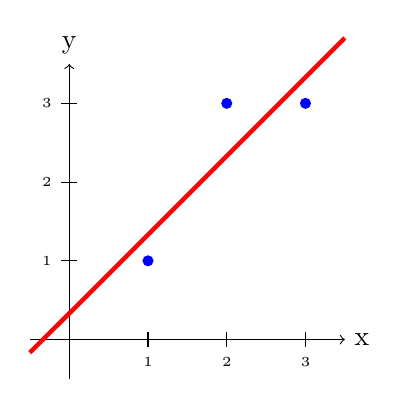
\begin{tikzpicture}
	% les axes
	\draw[->] (-0.5,0) -- (3.5,0) node[anchor=west]{x};
	\draw[->] (0,-0.5) -- (0,3.5) node[anchor=south]{y};
	\fill [blue] (1,1) circle (2pt);
	\fill [blue] (2,3) circle (2pt);
	\fill [blue] (3,3) circle (2pt);
	\draw[-] (1,-0.1) node[anchor=north]{\tiny 1} -- (1, 0.1);
	\draw[-] (2,-0.1) node[anchor=north]{\tiny 2} -- (2, 0.1);
	\draw[-] (3,-0.1) node[anchor=north]{\tiny 3} -- (3, 0.1);
	\draw[-] (-0.1,1) node[anchor=east]{\tiny 1} -- (0.1, 1);
	\draw[-] (-0.1,2) node[anchor=east]{\tiny 2} -- (0.1, 2);
	\draw[-] (-0.1,3) node[anchor=east]{\tiny 3} -- (0.1, 3);
	\draw[-,ultra thick, red] (-0.5,-0.167) -- (3.5,3.83);
	\end{tikzpicture}
\end{minipage}
\end{center}

\subsection{Généralisation à d'autres types de courbes}

Exprimée sous forme matricielle, l'équation \refeq{eq:regression}, 
 peut être utilisée non seulement
pour trouver la meilleure droite passant par un certain nombre de points, mais pour
beaucoup d'autre types de fonctions.  Supposons par exemple que l'on
veuille trouver la meilleure parabole décrivant les points
$(x_1, y_1), (x_2, y_2), \ldots, (x_n, y_n)$, c'est-à-dire qu'on cherche
les valeurs pour $a_0, a_1, a_2$ de l'équation 
\[
y = a_0 + a_1 x + a_2 x^2
\]
Dans ce cas-ci, on aura
\[
\matA = \begin{pmatrix}
a_0 \\ a_1 \\ a_2
\end{pmatrix}
\qquad,\qquad
\matY = \begin{pmatrix}
y_1 \\ y_2 \\ \vdots \\ y_n
\end{pmatrix}
\qquad,\qquad
\matM = \begin{pmatrix}
1 & x_1 & x_1^2 \\
1 & x_2 & x_2^2 \\
\vdots&\vdots&\vdots\\
1 & x_n & x_n^2
\end{pmatrix}
\]
qu'on substituera dans l'équation
\[
\transp{\matM} \matY =  \transp{\matM}\matM\matA 
\]
qu'on peut résoudre pour $\matA$ en utilisant la procédure d'élimination de Gauss-Jordan.
On peut généraliser ceci pour toute fonction pour laquelle on a un somme de termes
dont les coefficients sont à déterminer, comme par exemple,
$y = a_0 + a_1 \sqrt{x} + a_2 \sin x + \ldots$  On procéderait comme ci-dessus, sauf
qu'on utiliserait
\[
\matM = \begin{pmatrix}
1 & \sqrt{x_1} & \sin x_1^2 & \ldots \\
1 & \sqrt{x_1} & \sin x_2^2  & \ldots\\
\vdots&\vdots&\vdots\\
1 & \sqrt{x_1} & \sin x_n^2 & \ldots
\end{pmatrix}
\]

Par contre, on ne pourrait pas utiliser cette méthode directement pour résoudre
des équations dont les inconnues ne seraient pas des termes linéaires, comme
par exemple pour une gaussienne.
\[
y = a_0 e^{-a_1 x^2}
\]

Cela dit, nous ne sommes pas restreint à faire des régressions dans le plan.  
Supposons que nous ayons des triplets de points de la forme $(x,y,z)$ et que l'on
veuille déterminer le meilleur plan qui approxime ces points.
On n'aurait qu'à écrire
\[
z = a_0 + a_1 x + a_2 y
\]
et à procéder comme ci-dessus.
